\chapter{Introduction}

This document constitutes our efforts to organize a body of work concerning the development of spatial music instruments, software/hardware, and XR frameworks, which can jointly be used for musical experiments. The focus of this work is to use open source and low-cost solutions which might allow for greater proliferation of spatial music and easier reproduction of these works in the years to come. In this work we will talk about the history of pioneering composers of \textit{spatial music} and discuss at length what available systems exist to for the creation, documentation and dissemination of these works.

\section{Physics of Sound}

\section{Auditory System}

\section{Art of Spatial Sound}

Space as a parameter of music-making is a feature which has been explored by composers for hundreds and hundreds of years. Unfortunately, most musicians have a limited understanding of the possibilities that modern systems provide them and continue to operate on the basis of two-dimensional sound\footnote{Left/right panning plus distance modeled via amplitude changes or the addition of reverberation.}. Despite gargantuan efforts by the industry to expand commercial audio systems from stereo to more sophisticated formats, two-channel audio reproduction has remained the \textit{de facto} playback method in most homes due to their accessibility and simplicity. 

Prior to electro-acoustic composers, many artists experimented with space as a parameter of composition by including within their scores: the placement of musicians in different parts of the concert hall, choreographed trajectories for musicians, or using height by placing musicians in balconies. Many challenges which existed then remain now: synchronicity between players, architectural changes between venues, or providing a consistent experience for all audience members regardless of their seat.

Avant-garde composers in the 20th century pushed the envelope further by taking advantage of the technological developments of their era. With the advent of transmitted and recorded sound, \textit{disembodied sound} - a musicological term referring to the displacement in space-time of musician and sound - found a permanent role in the \textit{acousmatic} works of: Schaeffer, Xenakis, and Cage, to name a few. These \textit{acousmatic} works, meant for reproduction over loudspeakers, made great use of spatial audio technologies such as the \textit{quadraphonic} or \textit{octophonic} sound systems\footnote{Four and eight channel sound systems, respectively.}, which were being developed at the time.

Unfortunately, despite great scientific leaps, many of these older works cannot be fully appreciated by the general public since these high-end sound reproduction systems remain protected by privileged institutions, and commercial movie theatres, which harbor similar systems, have no financial incentive to reproduce these works. Part of the motivation of this thesis is to explore accessible techniques for the creation, documentation, and dissemination of works which employ spatial sound as a primary component of the compositional process. 

While many composers today, in well-funded contexts, have the pleasure to explore spatial sound through the use of multi-channel systems, much of their detailed work commonly gets \textit{down-mixed}\footnote{Compressed down from a multi-track format to stereo, usually for commercial purposes.} to stereo formats. If the spatial attributes of a particular sound are indeed important to the composition, this ultimate representation leaves much to be desired. Luckily, many free and open-source solutions exist for audio engineers to create and re-distribute works of this variety preserving the environmental auditory elements pertinent to the works.

In addition to discussing technologies available for the creation, recording, and presentation of 3D audio, in a musical context, we will discuss some of the inherent technical challenges inherent in these productions. Namely, we will consider the difficulty of 3D sound reproduction based on computer: storage, speed, and changing operating systems (OS). We hope this work is useful for any composer interested in the minutiae of the science, and art, of \textit{spatial music}.

\section{Psycho-acoustics of Spatial Sound}

Before we can understand the mathematical details behind different 3D audio technologies\footnote{3D audio is another name given to the field of spatial audio. In musical domain we often refer to this practice as sound \textit{diffusion}.}, we should discuss some of the psycho-acoustic principles on which all spatial audio technologies rely. Many authors have extensively written about the subject, with entire books having been dedicated to the subject, Blauert's 1997 \cite{blauert1997spatial} being the most popular. Here we will give only a short account of the many experiments that have been undertaken on the subject in order to inform the reader of some of the most salient features of the auditory system, which inform our perception of sounds in space.

From the psycho-acoustic perspective perhaps the most important feature of the auditory system is our ability to localize sound, which is why so much attention has been devoted to the subject. We can easily see how having a sensitive auditory localization system would be an evolutionary advantage. Being able to detect the presence of a predator, before it can reach us, is likely why we have developed the ability to localize sound. Similarly, being able to detect prey, before it can escape, would be evolutionarily advantageous.

A number of perceptual mechanisms work in conjunction and amalgamate into a single sensory experience which informs our understanding of sound direction. Not only are we conditioned to use acoustic cues to draw these conclusions, but memory and vision also form a part of this complex model. Our subconscious has a mental map of the prevailing origin of different sounds based on prior experience, which informs our predictions. For example, we seldom hear birds chirping below us because they generally fly above our heads, or rest on branches that are higher than us. As such, you will seldom see someone searching for a bird below them. Similarly, if you momentarily perceive that same bird to indeed be below you, you will likely confirm, or refute, this suspicion by gazing at that direction, and adapt your understanding based on the confluence of sensory information. 

In the acoustic domain, however, is where we find the greatest number of auditory cues responsible for our discernment of sound direction. Our auditory model of sound localization is indeed quite complex, especially for multiple sources in spaces. When sound waves travel through air, if there is more than a single source, the pressure waves might constructively and destructively interfere\footnote{Constructive and destructive interference refers to pressure waves' ability to increase or decrease in amplitude based on interactions with each other. For example, a negative pressure anti-node might perfectly cancel a positive pressure anti-node when two waves of equal frequency are offset in phase by 180\textdegree.}, making position estimations harder. Additionally, if the space is very \textit{reverberant}, if there are many reflections from walls, such as in a chapel, these predictions might become even more complicated to make.

It is useful within this scope distinguish between source localization of \textit{near-field} and \textit{far-field} sources. As their names suggest, \textit{near-field} sources are those that are proximal and \textit{far-field} sources are those which are relatively distant from us. These definitions have real world implications, namely, \textit{near-field} sources will arrive at our ears before any reflections muddle our perception of sound direction arrival. In contrast, \textit{far-field} sources will produce complex spectra, as reflections and \textit{direct sound} might interact in unpredictable ways. 

In this context, it is useful to further define two common conditions for sounds sources, those in \textit{free-fields} and those in \textit{diffuse-fields}. \textit{Free-field} refers to an environment in which there is no reverberation, in other words, there are no surfaces upon which the sound may reflect. This condition is seldom found in nature, however \textit{anechoic chambers}, rooms with no echoes, such as the one in Figure \ref{fig:ibm-anechoic}, have been designed specifically for the purpose of acoustic experiments. In contrast, a \textit{diffuse-field} refers to a condition in which prominent reflections are present, ideally with equal energy arriving from all directions. In architectural acoustics, diffusion will often be introduced intentionally, such as in concert halls, in order to spread energy evenly across the entire listening space. In between these two extremes there exists a spectrum of situations, each with their own acoustic characteristics, such as the: \textit{reverberation time} (T60) of the room, or the shortest reflection path from a source to a subject, whether that be a person or a receiver.

\begin{figure}[ht!]%force figure here, top, strict
\centering
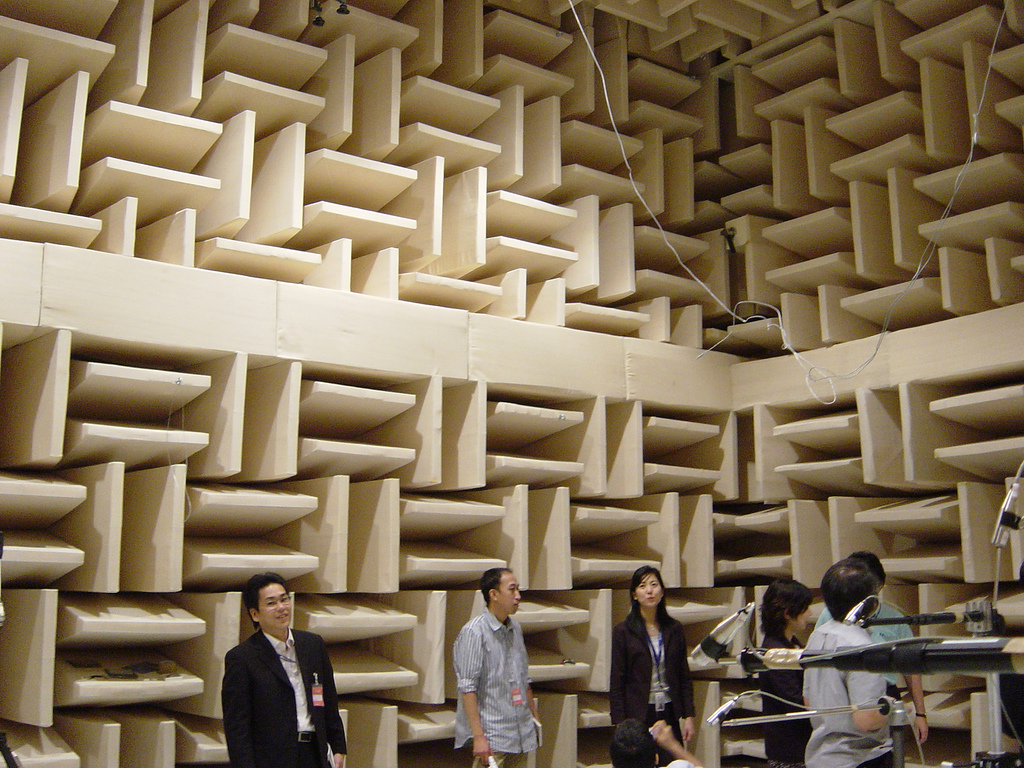
\includegraphics[width=0.6\textwidth]{img/ibm-anechoic.jpg} 
%\captionsetup{justification=centering}
\caption{IBM Anechoic Chamber - wikimedia commons}
\label{fig:ibm-anechoic}
\end{figure}

\subsection{HRIRs}\label{subsec:hrirs}

An important aspect of spatialization in the musical domain, in addition to horizontal and vertical direction of sounds, is the distance of the event in relation to listener. For these three critical localization parameters - those being horizontal position, vertical position, and distance - various associated auditory mechanisms exist in the acoustic domain which facilitate our ability to place sources in space. 

In \textit{near-field} conditions, \textit{auralization} systems - systems that seek to replicate natural phenomena via digital means - tend to model distance as an independent characteristic of directional acoustic propagation. A common definition of \textit{near-field}, albeit informal, is: anything within arms reach, or between 0.5m and 1m (\cite{Betbeder.2017})\footnote{1-2m is the typical distance for HRTF measurements.}. The idea behind this formal separation of near and far field is to exploit "tricks" in sound system design which help simulate real-world acoustic conditions at a much lower computational cost. By analyzing real-world acoustic snapshots, taken with microphones as \textit{impulse responses} (IR) we can observe that many acoustic spaces exhibit similar behaviors, statistically, in particular regions of their \textit{impulse responses}. 

Any acoustic space can be considered a linear time-invariant (LTI) system which can be characterised by a single \textit{impulse response}, much like any other digital filter. Subtle changes in air pressure, based on temperature for example, can affect sound propagation, but for all intents and purposes, this theory holds true. Inside this \textit{near-field} the abundance or lack of reverberant sound, caused by reflections from surfaces, can contribute to our perception of sound distance. However, it is more common to model the \textit{diffuse-field} attributes independently, and use a complimentary system, based on \textit{free-field} plus \textit{near-field} techniques, for horizontal and vertical \textit{auralization}.

Within this particular context, our free/near field condition, we are concerned with impulse responses not of a single omni-directional acoustic sensor, for spatialization systems, but rather with the analysis of two impulse responses - ideally captured at the listeners ears. For this purpose there exist various methodologies for capturing the aforementioned impulse response commonly referred to as \textit{binaural impulse responses} (BIRs) or \textit{Head Related Impulse Responses} (HRIRs), in the time domain\footnote{When these are taken in diffuse-field conditions they are also sometimes called Binaural Room Impulse Responses (BRIRs).}. The most common technique involves placing two small microphones, or \textit{in-ear} microphones, inside a persons ears, and taking snapshots at as many positions as possible by sending \textit{exponential sinusoidal sweeps}\footnote{One among various IR capture methods including: balloon pops, MLS, and linear sinusoidal sweeps.} from speakers surrounding the listener. 

The recordings are then \textit{de-convolved} in order to obtain the effect only of the listeners head and body on the two recordings, as a function of direction. When the excitation signal is perfectly known, de-convolution yields an impulse response which captures the effects of the: room, speaker and microphone. A full-spectrum signal is required for a good IR to be obtained. We tend to use \textit{flat} frequency microphones and speakers, and an anechoic chamber, which has no response, to isolate the effects of head and torso on the incoming signals.

\begin{figure}[ht!]%force figure here, top, strict
\centering
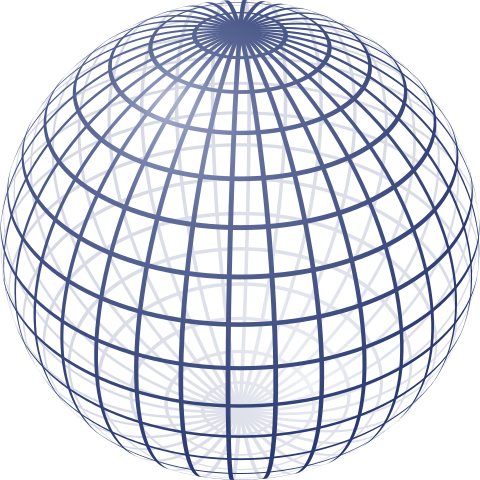
\includegraphics[width=0.3\textwidth]{img/sphere-png.png} 
%\captionsetup{justification=centering}
\caption{Sphere - wikimedia commons}
\label{fig:sphere}
\end{figure}

Figure \ref{fig:sphere} shows a spherical grid, included here to facilitate visualization of the proposed acoustic system. Consider a speaker at each junction between two lines and a listener with \textit{in-ear} microphones in the center of the sphere. The acoustic sampling of the sphere, in the \textit{binaural} sense, will take place by taking \textit{impulse responses} with each speaker, two at a time - one for each ear. This complete set of HRIRs, taken in \textit{free-field} conditions, such as inside our \textit{anechoic chamber}, contain time, level and spectral differences used by our auditory system to localize sound. 

Each of these individual characteristics of each HRIR has a particular name. \textit{Inter-aural level difference} (ILD) refers to the overall energy difference between the two IRs, \textit{inter-aural time difference} (ITD) refers to the time offset, or phase delay, between measurements. Based on the \textit{diffraction}\footnote{Diffraction refers to sounds ability to bend around objects. This is especially true for low frequencies.} and \textit{reflection}\footnote{Reflection refers to sounds ability to bounce off objects. This is especially true for high frequencies.} effects caused by the geometry of the human head, the HRIRs will also exhibit spectral differences, which can be used to discern directions in situations when ITDs and ILDs are not sufficient. ILDs are typically caused by the \textit{shadowing effect} of the head and are therefore frequency dependent (\cite{cuevas20193d}). In other words, the ILD will be greater for higher frequencies since lower frequencies diffract, or bend, around the head, while high-frequencies reflect off the head. 

\subsection{Localization Errors}

Many terms have been defined in the psyscho-acoustic community to describe common occurrences in auditory experiments. Our ability to localize sounds is greatly dependent on the nature of the acoustic environment, as well as the frequency content of the sound source. In addition, we should remember that in the real world, more often than not, multiple sound sources will be present at the same time, making localization tasks more difficult still.

\begin{figure}[ht!]%force figure here, top, strict
\centering
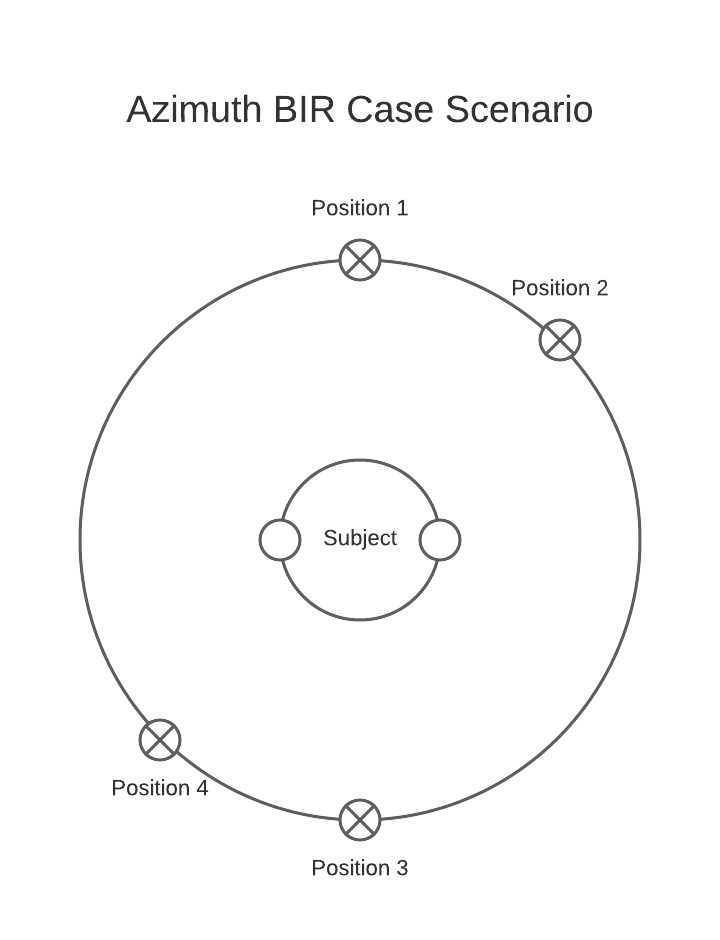
\includegraphics[width=0.5\textwidth]{img/azimuth-bir.png}
%\captionsetup{justification=centering}
\caption{Azimuth BIR Case Scenario}
\label{fig:azimuth-bir}
\end{figure}

In order to demonstrate some common localization errors, we present figure \ref{fig:azimuth-bir}. Consider positions 1 and 3 the figure. Clearly these two positions on the \textit{transverse} plane, otherwise known as the horizontal plane, have identical ILDs and ITDs since the distance from both positions to the subject's ears is identical. Therefore, the subject will only be able to rely on spectral differences to localize the impinging sound. Our outer ear, or \textit{pinna}\footnote{Also called the auricle in some medical textbooks.}, blocks high frequencies arriving from behind the listener acting as low-pass filters. The HRIRs capture all these time and frequency differences in order to simulate directionally-dependent sound propagation via convolution of the associated IRs. 

In contrast, differentiating between positions 2 and 4 should be substantially easier, since we see that the ITD and ILD differences will compliment spectral changes giving us additional information. Assuming the subject is facing position 1, the distance between position 2 and the subjects right ear, the \textit{ipsilateral} ear\footnote{The ear closest to the source.}, will be smaller than the distance to the \textit{contralateral} ear\footnote{The ear furthest away from the source.}. Sound propagates in air at a rate of around 343 m/s and as it travels it loses energy due to friction between molecules according the inverse-square law\footnote{The inverse square law states that with every doubling of distance away from the sound source, the sound will be four times less intense.}. 

\begin{figure}[ht!]%force figure here, top, strict
\centering
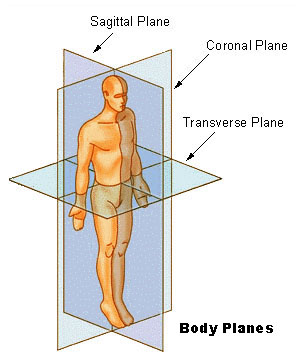
\includegraphics[width=0.5\textwidth]{img/body-planes.jpg}
%\captionsetup{justification=centering}
\caption{Body Planes - wikimedia commons}
\label{fig:body-planes}
\end{figure}

This additional distance results in a time delay between IRs, as well as level differences. However small these differences might seem, they are crucial for discerning the position of sounds in space. The inability of listeners to differentiate between two sources with identical ITDs and ILDs, that is: any two sources mirrored over the coronal plane\footnote{Also called the frontal plane.}; is called \textit{front-back confusion}. The same principle applies to sources mirrored over the \textit{transverse plane}\footnote{Also called the horizontal plane.}, these errors are called \textit{up-down confusions}. Sources mirrored over the \textit{mid-sagittal}\footnote{Also known as the longitudinal or median plane.} should be easily discerned since ILDs and ITDs will be quite large.  

The human auditory system has been shown to be extremely sensitive. The ITD for a typical human head can vary between $\pm$750$\mu$s. Humans can detect ITDs as low as 10-20$\mu$s which correspond to about 1\textdegree in the horizontal plane (\cite{hacihabiboglu2017perceptual}). ITDs are commonly held as the primary localization cues for low frequencies, while ILDs are more prominent for high frequency signals. 

\begin{figure}[ht!]%force figure here, top, strict
\centering
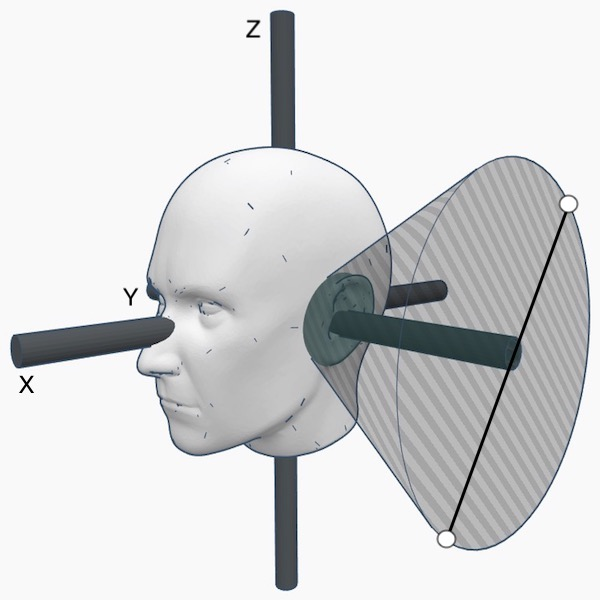
\includegraphics[width=0.5\textwidth]{img/cone_confusion.JPG}
%\captionsetup{justification=centering}
\caption{Cone of Confusion}
\label{fig:cone-confusion}
\end{figure}

The \textit{cone of confusion} is yet another term used to describe a phenomenon generally experienced in localization experiments. Consider the two white dots on the circumference of the cone depicted in figure \ref{fig:cone-confusion}. The two positions, much like any two dots directly opposite each other on this circle, will have identical ITDs and ILDs because their respective distances to the \textit{contralateral} and \textit{ipsilateral} ears, will be the same. In this cases, spectral differences become critical to differentiate between sources. When ambiguous localization tasks arise, small head movements often help resolve source positions.

Our ability to localize sources is most accurate in the horizontal plane. Psycho-acoustic experiments have revealed that \textit{localization blur}, the inability for listeners to discern the direction of a sound, is generally less than 10\textdegree for horizontal sources, but around 20\textdegree for sources in the median plane (\cite{hacihabiboglu2017perceptual}). Two associated objective measures are the \textit{Minimum Audible Angle} (MAA) and the \textit{Minumum Audible Movement Angle} (MAMA). The MAA, a formal term used to quantify \textit{localization blur}, is the minimum detectable angular difference of two successive sound sources \cite{reardon2017evaluation}. The MAMA, is the smallest arc that a moving source must travel to be discriminable from a stationary source \cite{moore1995hearing}.

\subsection{Perception of distance}

Perception of distance is more complex in some ways than that of orientation. \cite{zahorik2005auditory} provides, a comprehensive overview of auditory distance perception research, including some cognitive research which examines brain response to acoustic stimuli. As aforementioned, there are several cues that affect our perception of distance - the most salient one being overall energy. A few other unmentioned cues, however, also affect our perception of distance. Among these, is the absence, or presence, of high frequency content in a signal. High frequency signals tend to dissipate faster in air than low frequency ones, because of the additional friction between molecules inherent to these acoustic events. 

\textit{Auditory parallax}, the effect whereby the position or direction of an object appears to differ when heard from different positions, has also been shown to improve distance estimations. Finally, as mentioned before, familiarity tends to affect our perception of sound origin. A sample of a whispering voice, virtually placed far away, will appear closer than it really is. Adversely, a shouting voice, placed close, will appear to be further away than reality.

Finally, \textit{interaural coherence} (IC), is the measured statistical coherence of signals received at each ear. In a \textit{diffuse field}, IC is low, because the scattering of sounds off walls interact in unpredictable ways, which result in some amount of randomness in the signals when compared to each other. Therefore, IC can be used as a statistical estimate of distance since we can assume that in most real-world conditions sound sources will be diffused acoustically lowering the overall IC for distant sources more than those proximal.

\subsection{Precedence effect}

\textit{Summing localization} is a phenomenon - primarily based on ITD - which affects of perceived direction-of-arrival of sounds. When a broadband signal - a signal with broad range of frequencies present - is played from two directions with a small delay of less than 1 ms, a single event is perceived at the direction between sources. The perceived location shifts towards the first played source, as the delay increases. This \textit{fusion} is one of three characteristics of the \textit{precedence effect}, also known as the \textit{Law of First Wavefront} or \textit{Haas effect}, described in 1949 by Helmut Haas. When the delay is between 1 and 5ms, a single event close to the leading source can be heard \cite{hacihabiboglu2017perceptual}. The lagging source - the delayed copy of the sound - can be perceived due to the change in timbre, and is essentially equivalent to a feedforward comb filter where the delayed copy is played back over a second discrete channel. Within this context the \textit{echo threshold}, refers to the amount of delay that must be introduced to the copy before we begin perceiving the two sounds as independent non-fused events. This threshold is dependent on the nature of the signal. For a short broadband click, 5 ms might be enough to create an echo. For music and speech signals, the threshold is longer, and can be as high as 20 ms.

The precedence effect can be summarized by the following three phenomena: 

\begin{enumerate}
    \item \textit{Localization dominance}: the direction of an auditory event depends predominantly on the leading source.
    \item \textit{Fusion}: a single auditory event is perceived when two sound events are below the \textit{echo threshold}.
    \item \textit{Lag Discrimination Suppression}: the direction of the lagging sound is suppressed.  
\end{enumerate}

\subsection{Binaural Synthesis}

Of particular importance to our work is the use of binaural synthesis for the simulation of acoustic spaces. Binaural synthesis allows us to experiment with \textit{spatial music} without the need for sophisticated and often inaccessible loudspeaker systems. In binaural synthesis, sound sources are \textit{convolved}\footnote{Convolution of a source with an impulse response if equivalent to applying a filter.} with HRIRs dynamically to simulate surround sound experiences. Binaural synthesis has become increasingly popular with the growth of \textit{extended reality} (XR) systems. Several problems, such as: personalized HRTFs, externalization problems, and localization errors; persist. 

Poor \textit{externalization}\footnote{Also sometimes refered to as Inside-the-Head Locatedness (IHL).}, the degree to which listeners perceive sources as originating inside their head, can be mitigated by the use of a head-tracking system. The systems, based on \textit{inertial measurement units} (IMU), monitor the orientation of the listener and adjusts the soundfield accordingly - ideally in real-time. When no rotation adjustment is included, our auditory system assumes that sources must be originating from inside our head, as this is the only rational conclusion for sources without dynamic filtering based on BIRs. The subtle spectral changes from location to location, provided by head-tracking, provide a way to disambiguate between source positions. The addition of diffuse field modeling, in the form of reverberation unit, also supports improved \textit{externalization}(\cite{sakamoto1976out}). 
%%%%%%%%%%%%%%

\cite{cuevas20193d} provides an extensive literature review on the subject of \textit{binaural spatialization}. In this particular text, one of the most comprehensive readings on binaural synthesis, the authors describe the steps undertaken for each part of the "signal chain". Figure \ref{fig:3dti-chain} shows a diagram of the implementation. 

For the \textit{free-field} modeling, an anechoic system based on BIRs/HRIRs is implemented, following:

\begin{enumerate}
    \item Distance-dependent attenuation (inverse square law or acoustic power law), this step also includes far-field distance simulation modeling air impedance (distance-dependent low-pass filtering).
    \item HRIR obtained using \textit{barycentric interpolation} and are ITDs removed to dynamically adjust for different head sizes.
    \item HRIR convolution.
    \item ITD is computed and added to the signals.
    \item ILD correction for \textit{near-field} sources.
    \item Directionality features for hearing aids (if any).
\end{enumerate}

For the \textit{diffuse-field} modeling, an non-anechoic system based on BRIRs is implemented, following:

\begin{enumerate}
    \item Independent distance-dependent attenuation to control the \textit{direct-to-reverberant ratio} (DRR). 
    \item Sources are encoded into 1st Order Ambisonic (FOA).
    \item These channels are convolved with encoded versions of the BRIRs, which have been processed to remove any direct sound.
\end{enumerate}

\begin{figure}[ht!]%force figure here, top, strict
\centering
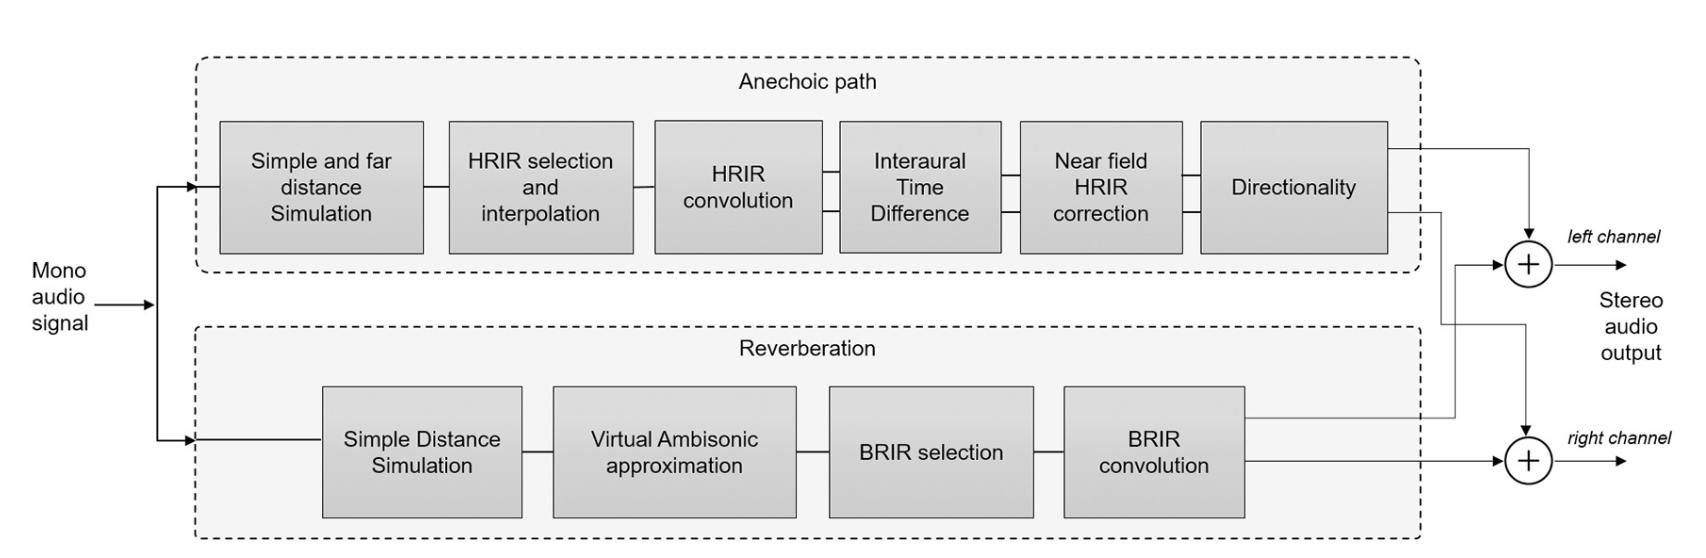
\includegraphics[width=1.0\textwidth]{img/3dti-chain.png} 
%\captionsetup{justification=centering}
\caption{3DTI Toolkit Binaural Structure - \cite{cuevas20193d}}
\label{fig:3dti-chain}
\end{figure}

%free vs. diffuse field

\subsection{Reverberation}
%dont forget to talk about room acoustics. T60, etc. Sabine equation. RT60. 

%near, far



%https://books.google.com.bo/books?id=OywDx9pxCMYC&pg=PA1&source=gbs_toc_r&hl=es-419#v=onepage&q&f=false






\section{Conclusion}